\section{Introduction}


% \begin{frame}

%   % Application pictures
% \end{frame}

% \begin{frame}{Text Generation}

%   \[ \argmax_{y_{1:T}} f(y_{1:T} ; x, \theta)\]

% \end{frame}

\begin{frame}{Machine Learning for Natural Language}
  What types of models get used for this equation? 


  \[\argmax_{y_{1:T}} \alert{f}(y_{1:T}, x; \alert{\theta}) \]

\end{frame}

\begin{frame}{State-of-the-Art Natural Language Processing, circa 2009}

  % Picture
  \begin{center}

    \scalebox{0.8}{
  \begin{tikzpicture}[node distance=0.2cm]
    \node(task)[minimum height=2em] {\textbf{Task} $(x, y)$};
    \node(aa) [draw, rounded corners, minimum width=12em,minimum height=3em, below= of task]{Syntax};
    \node(bb) [draw, rounded corners, minimum width=12em,minimum height=3em, below= of aa]{Surface Structure};
    \node(cc) [draw, rounded corners, minimum width=12em,minimum height=3em, below= of bb]{Translation};
    \node(dd) [draw, rounded corners, minimum width=12em,minimum height=3em, below= of cc]{Summarization};
    \node(ee) [draw, rounded corners, minimum width=12em,minimum height=3em, below= of dd]{Coreference};
    \node     [below= of ee]{$\vdots$};


    \visible<2>{
    \node(model) [minimum height=2em, right= of task, xshift=5cm]{\textbf{Model Class} $f(\cdot; \theta)$};
    \node(a) [draw, rounded corners, minimum width=10em, minimum height=3em, below= of model]{Parsing};
    \node(b) [draw, rounded corners, minimum width=10em, minimum height=3em, below= of a]{CRF Tagging};
    \node(c) [draw, rounded corners, minimum width=10em, minimum height=3em, below= of b]{Alignment EM};
    \node(d) [draw, rounded corners, minimum width=10em, minimum height=3em, below= of c]{Logistic Regression};
    \node(e) [draw, rounded corners, minimum width=10em, minimum height=3em, below= of d]{Language Modeling};
    \node [below= of e]{$\vdots$};

    \draw (aa.east) -- (a.west);
    \draw (aa.east) -- (b.west);
    \draw (bb.east) -- (b.west);
    \draw (bb.east) -- (e.west);
    \draw (cc.east) -- (c.west);
    \draw (cc.east) -- (e.west);
    \draw (dd.east) -- (a.west);
    \draw (dd.east) -- (c.west);
    \draw (dd.east) -- (e.west);
    \draw (ee.east) -- (a.west);
    \draw (ee.east) -- (b.west);
    \draw (ee.east) -- (c.west);
}
  \end{tikzpicture}
}
  \end{center}
\end{frame}

\begin{frame}{State-of-the-Art Natural Language Processing, circa 2019}
\begin{center}
    \scalebox{0.8}{
  \begin{tikzpicture}[node distance=0.2cm]
    \node(task)[minimum height=2em] {\textbf{Task} $(x, y)$};
    \node(aa) [draw, rounded corners, minimum width=12em,minimum height=3em, below= of task]{Syntax};
    \node(bb) [draw, rounded corners, minimum width=12em,minimum height=3em, below= of aa]{Surface Structure};
    \node(cc) [draw, rounded corners, minimum width=12em,minimum height=3em, below= of bb]{Translation};
    \node(dd) [draw, rounded corners, minimum width=12em,minimum height=3em, below= of cc]{Summarization};
    \node(ee) [draw, fill=red!10, rounded corners, minimum width=12em,minimum height=3em, below= of dd]{New Tasks};
    \node     [below= of ee]{$\vdots$};


   \visible<2->{
    \node(model) [minimum height=2em, right= of task, xshift=5cm]{\textbf{Model Class} $f(\cdot; \theta)$};
    \node(a) [draw, rounded corners, minimum width=10em, minimum height=3em, below= of model, yshift=-2.5cm]{Neural Networks};

    \node<3>[below=of a]{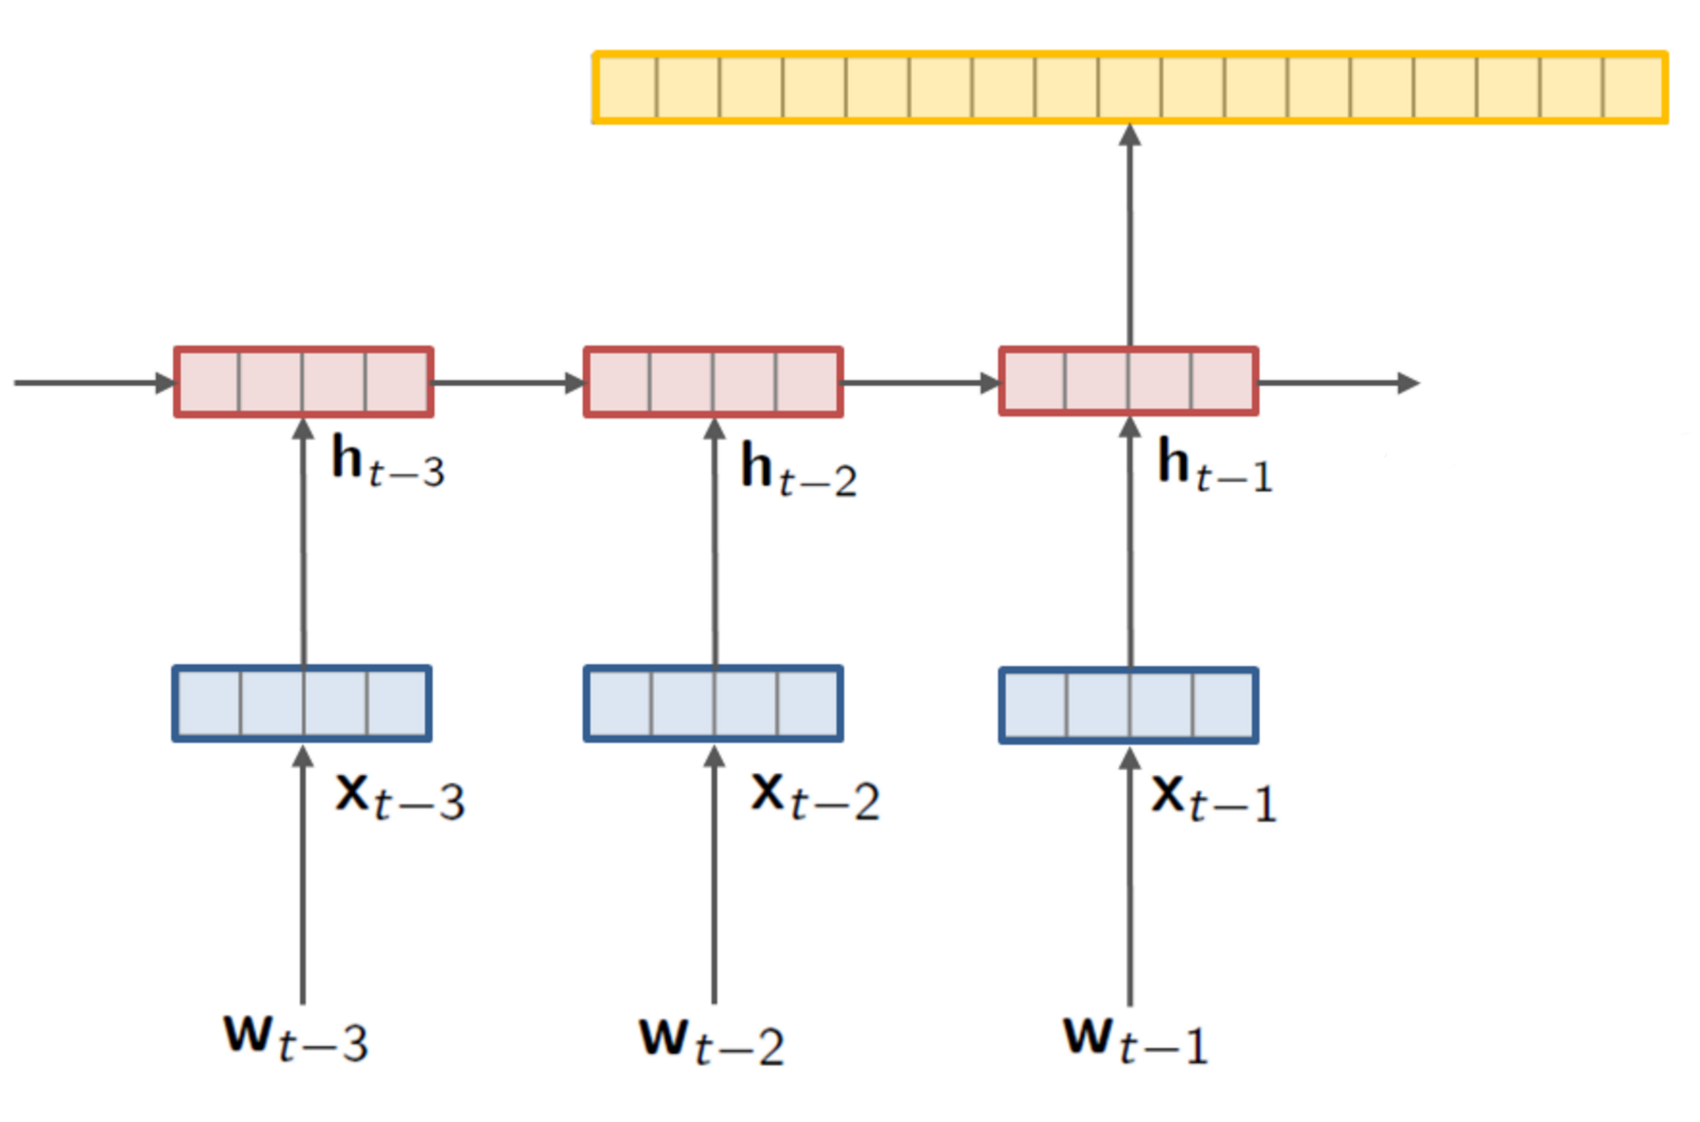
\includegraphics[width=4cm]{rnnlm6}};

    % \node[below  = of a, xshift=3cm]{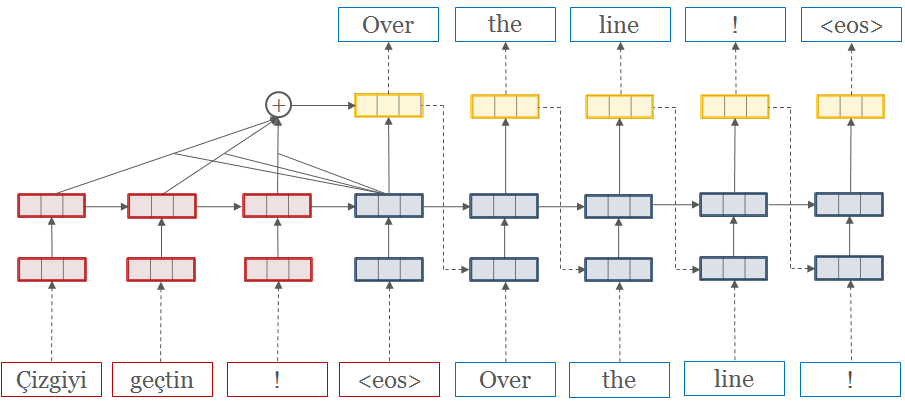
\includegraphics[width=8cm]{nmt}} ;

    % \node(b) [draw, rounded corners, minimum width=10em, minimum height=3em, below= of a]{CRF Tagging};
    % \node(c) [draw, rounded corners, minimum width=10em, minimum height=3em, below= of b]{Alignment EM};
    % \node(d) [draw, rounded corners, minimum width=10em, minimum height=3em, below= of c]{Logistic Regression};
    % \node(e) [draw, rounded corners, minimum width=10em, minimum height=3em, below= of d]{Language Modeling};
    \node [below= of e]{$\vdots$};

    \draw (aa.east) -- (a.west);
    \draw (bb.east) -- (a.west);
    \draw (cc.east) -- (a.west);
    \draw (dd.east) -- (a.west);
    \draw (ee.east) -- (a.west);
}

  \end{tikzpicture}
}


\end{center}
\end{frame}

% \begin{frame}{Performance}

% \end{frame}


% \begin{frame}

% \end{frame}

% \begin{frame}{Central}
%   % Picture
%   \begin{tikzpicture}
%     \node{};
%   \end{tikzpicture}
% \end{frame}


\begin{frame}{Harvard NLP Deep Learning Research}{}
  % Picture
  % \research{\cite{Deng2016}}

  \begin{center}
    \scalebox{2}{
  \begin{tikzpicture}

    \node<1> at (10mm, 15mm){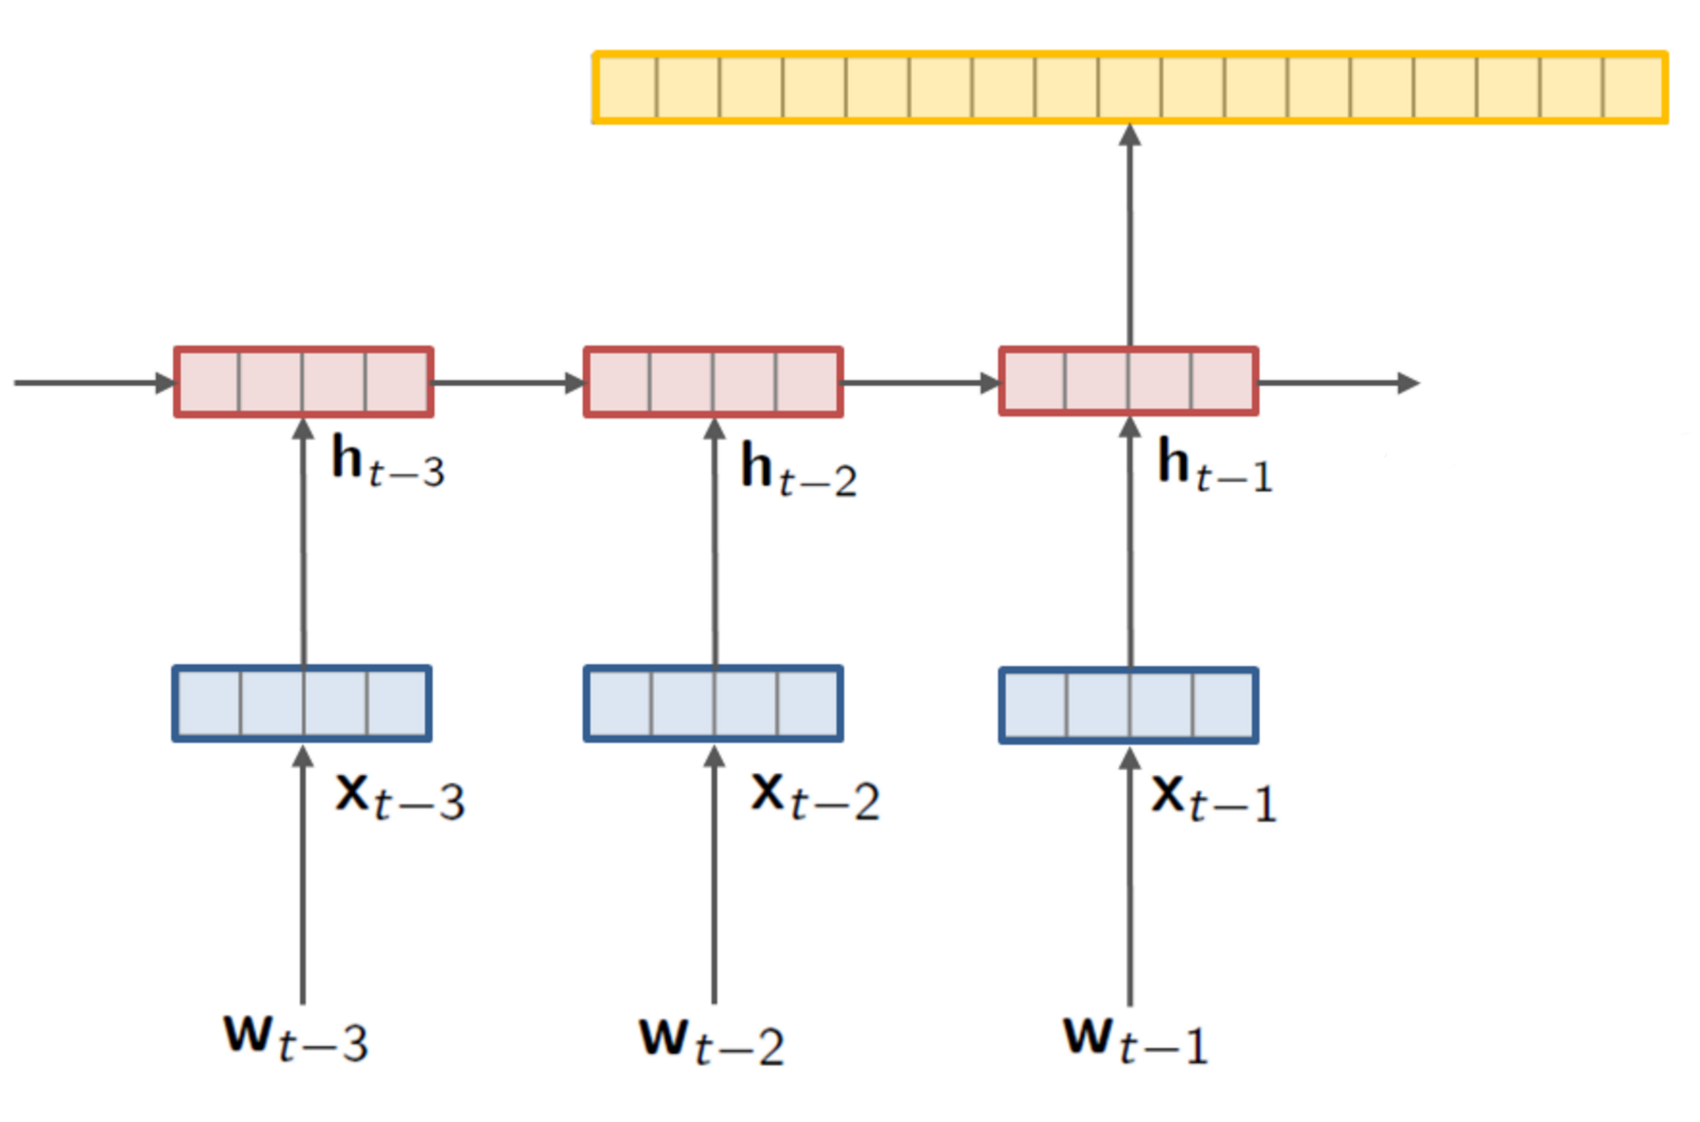
\includegraphics[width=3.4cm]{rnnlm6}};

    \node[draw,  thick, rounded corners, scale=0.5] (ana) at (-15mm, 15mm) {Analysis};
    \node[draw,  thick, rounded corners,scale=0.5] (meth) at (0mm, 30mm) {\ Methods\phantom{p}};
    \node[draw,  thick, rounded corners,scale=0.5] (app) at (25mm, 30mm) {Applications};
    \node<2>[draw,  fill=yellow, thick, rounded corners,scale=0.5] (app) at (25mm, 30mm) {Applications};
    \node<2>[scale=0.5, text width=50mm] at (12mm, 15mm) {\small \centering Translation, \\  Summary,  \\ Data-to-Text,  \\ Diagram-to-Text,  \\ $\vdots$};

    \node[draw, thick, rounded corners, scale=0.5] (und) at (35mm, 15mm) {Understanding};
    \node[draw, thick, rounded corners, scale=0.5] (dep) at (25mm, 0mm){Scaling};

    \node[draw,  thick, rounded corners,scale=0.5] (imp) at (0, 0) {Open-Source};

    \draw (ana) -- (meth) --(app) -- (und) -- (dep) -- (imp) -- (ana);

  \end{tikzpicture}
}
  \end{center}

\end{frame}


\begin{frame}{Selected Harvard NLP Deep Learning Research}{}
  % Pictured

  \vspace{-1cm}

  \begin{center}
  \begin{tikzpicture}

    \node at (10mm, 15mm) {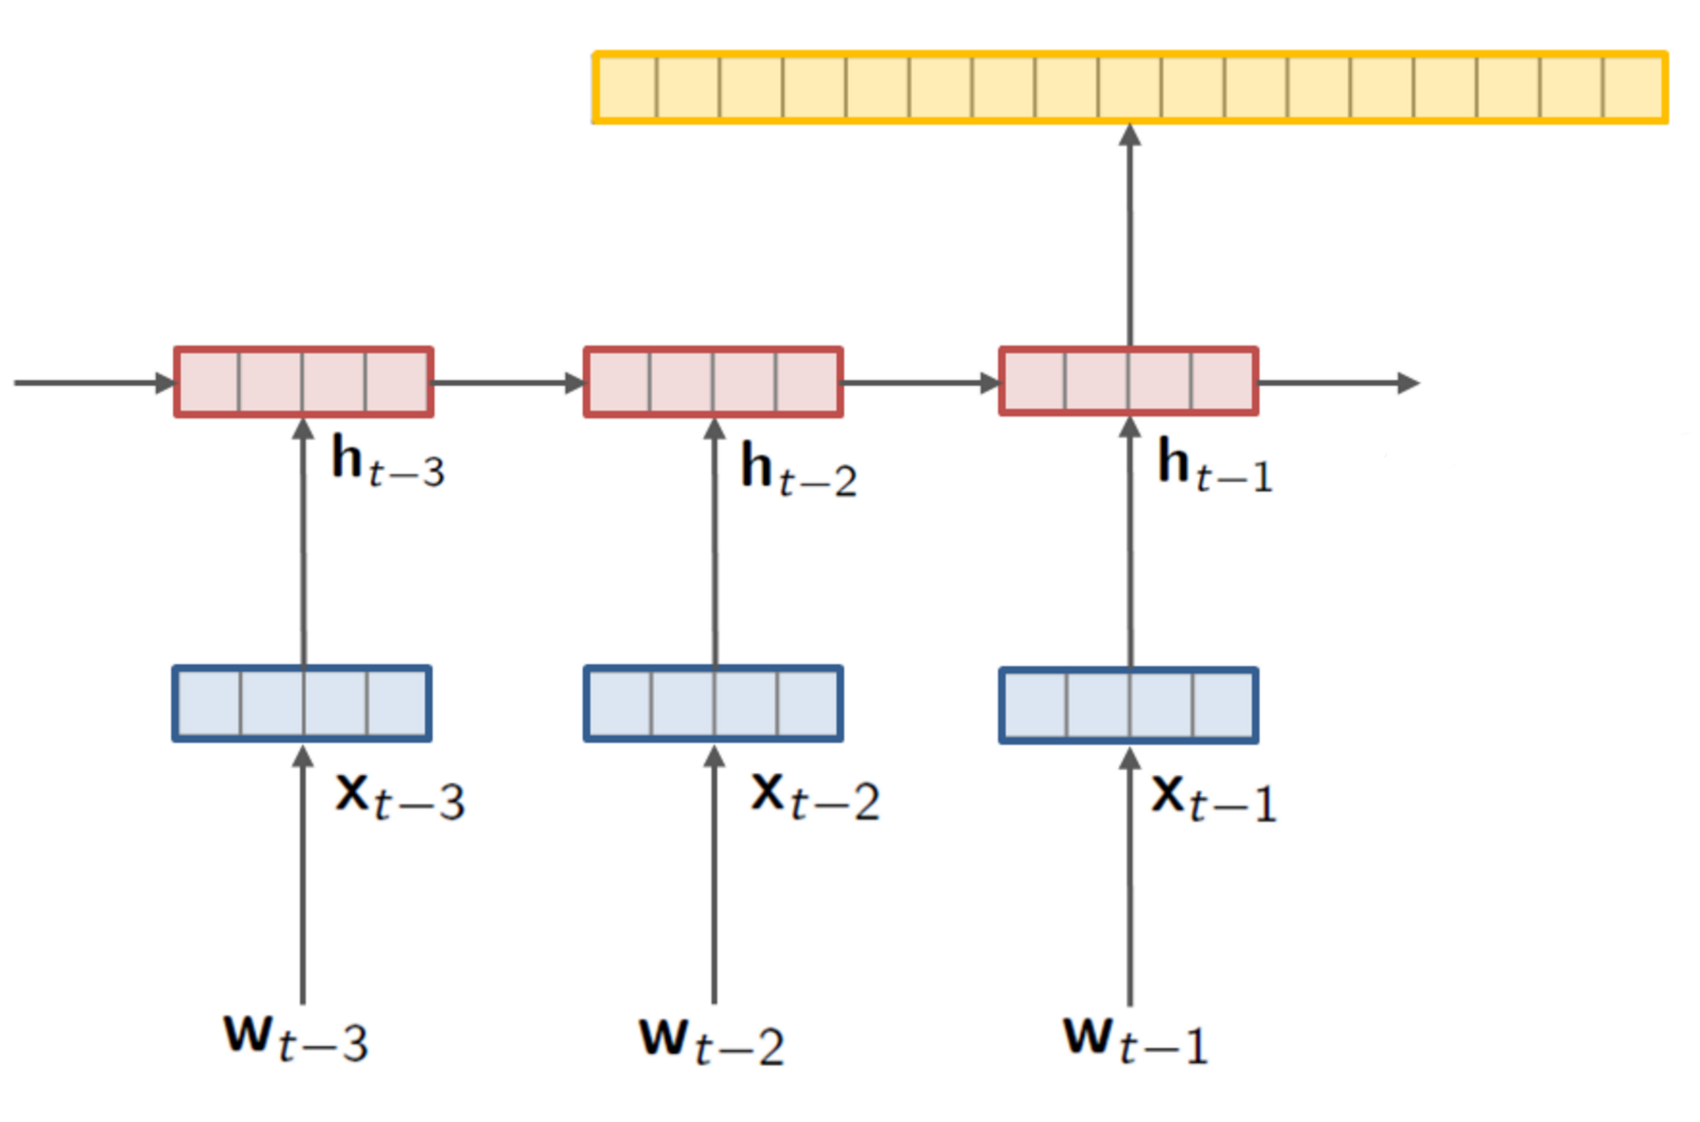
\includegraphics[width=2cm]{rnnlm6}};


    \node[rounded corners, draw] (ana) at (-15mm, 15mm) {Analysis};

    \visible<2,8>{
    \node at (-40mm, 15mm) [text width=30mm]{ \centering
      \baselineskip=-5pt  \scriptsize
      \structure{
      \citet{Strobelt2016}}
    \structure{
      \citet{strobelt2019s}}
      \citet{DBLP:conf/emnlp/WisemanSR17}
      \par
      };
    }

    \node[rounded corners, draw] (meth) at (0mm, 30mm) {\ Methods\phantom{p}};

    \visible<3,8>{
    \node at (-10mm, 35mm) [anchor=south, text width=30mm] { \centering

      \baselineskip=-5pt \scriptsize
      \citet{Kim2016} \ \
      \textcolor{red}{\cite{DBLP:journals/corr/KimDHR17}}\ \
      \cite{EMNLP2017}
      \par
      };
    }
    \node[rounded corners, draw] (app) at (25mm, 30mm) {Applications};

\visible<4,8>{

    \node at (35mm, 35mm) [anchor=south, text width=30mm]{ \centering
      \baselineskip=-5pt \scriptsize
      \citet{Rush2015}
      \textcolor{red}{\citet{Deng2016}}
      \citet{Schmaltz2016}
      \par
      };
}

    \node[rounded corners, draw] (und) at (35mm, 15mm) {Understanding};

\visible<5,8>{
    \node at (65mm, 15mm) [text width=30mm]{ \centering
      \baselineskip=-5pt \scriptsize
      \citet{wiseman2018learning}
      \textcolor{red}{\citet{deng2018latent}}\ \ \
      \textcolor{red}{\citet{DBLP:journals/corr/abs-1802-02550}}
      \par
      };
}

    \node[rounded corners, draw] (dep) at (25mm, 0mm){Scaling};

\visible<6,8>{
    \node at (35mm, -10mm) [text width=30mm] { \centering
            \baselineskip=-5pt \scriptsize
            \citet{Kim2016a}
            \citet{senellart2018opennmt}
            \alert{\citet{reagen2017weightless}}
            \par
      };
}
    \node at (75mm, -5mm) [draw, text width=35mm] {\centering
            \baselineskip=-5pt \scriptsize
            Natural Lang. Processing \\
            \alert{Machine Learning} \\
            \structure{Visualization}
            \par
      };


    \node[rounded corners, draw] (imp) at (0, 0) {Open-Source};
\visible<7,8>{
      \node at (-10mm, -10mm) [text width=30mm]{ \centering
        \baselineskip=-5pt \scriptsize
        \citet{DBLP:conf/acl/KleinKDSR17} \ \
        \citet{senellart2018opennmt} \ \
        \citet{rush2018annotated}
        \par
      };
}

    \draw (ana) -- (meth) --(app) -- (und) -- (dep) -- (imp) -- (ana);

  \end{tikzpicture}
  \end{center}
\end{frame}


% \begin{frame}{Talk Outline}
%   \begin{enumerate}
%   \item Research Direction 1: Applications
%   \item \alert{Research Direction 2: Analysis and Open-Source}
%   \item Research Direction 3: Methods and Scaling
%   \item Research Direction 4: Understanding
%   \end{enumerate}
% \end{frame}